\documentclass{beamer}
\usepackage{beamerthemeshadow}
\usepackage{verbatim}

\usepackage{lastpage}
\usepackage{xcolor}
\usepackage{pgf}
\usepackage{colortbl}
\usepackage{hyperref}

\newcommand{\bi}{\begin{itemize}}
\newcommand{\ei}{\end{itemize}}
\newcommand{\be}{\begin{enumerate}}
\newcommand{\ee}{\end{enumerate}}
\newcommand{\bd}{\begin{description}}
\newcommand{\ed}{\end{description}}
\newcommand{\prbf}[1]{\textbf{#1}}
\newcommand{\prit}[1]{\textit{#1}}
\newcommand{\beq}{\begin{equation}}
\newcommand{\eeq}{\end{equation}}
\newcommand{\bdm}{\begin{displaymath}}
\newcommand{\edm}{\end{displaymath}}

\newcommand{\ft}[1]{
  \frametitle{\begin{tabular}{p{4.2in}r} \textcolor{white}{#1} & \small{\insertframenumber / \inserttotalframenumber} \end{tabular}}
  %\frametitle{\begin{tabular}{p{4.2in}r} \textcolor{white}{#1} & \small{\insertframenumber / 7} \end{tabular}}
  \setbeamercovered{transparent=18}
}

\newcommand{\eft}[1]{
  \frametitle{\begin{tabular}{p{4in}r} \textcolor{white}{#1} & \small{\hyperlink{f:questions}{\beamergotobutton{GO BACK}}} \end{tabular}}
  \setbeamercovered{transparent=18}
}

\newcommand{\stepinv}{\setbeamercovered{invisible}}
\newcommand{\stopinv}{\setbeamercovered{transparent=18}}
\newcommand{\uncoverinv}[1]
{
  \setbeamercovered{invisible}
  \uncover<+->{#1}
  \setbeamercovered{transparent=18}
}
\newcommand{\ans}[1]{\textcolor{blue}{#1}}
\newcommand{\ansinv}[1]
{
  \setbeamercovered{invisible}
  \uncover<+->{\textcolor{blue}{#1}}
  \setbeamercovered{transparent=18}
}
\newcommand{\setinv}{\setbeamercovered{invisible}}
\newcommand{\setvis}{\setbeamercovered{transparent=18}}
\newcommand{\centerpic}[2]
{
  \begin{center}
  \includegraphics[#1]{#2}
  \end{center}
}
\newcommand{\h}[1]{\hat{#1}}
\newcommand{\ds}{\displaystyle}

%\definecolor{light}{rgb}{1.0,0.33,0.33}
\definecolor{light}{rgb}{1.0,0.5,0.5}
\newcommand{\hl}[1]{\alt<#1>{\rowcolor{light}\hspace*{-2.1pt}} {\hspace*{-2.1pt}} }

\definecolor{mycolor}{rgb}{0.6,0.0,0.0}
\usecolortheme[named=mycolor]{structure}

\title{A Life Insurance Deterrent to Risky Behavior in Africa}
\author[James Murray, Department of Economics]{Pedro de Araujo\\Department of Economics and Business\\Colorado College\\ \and\\ James Murray\\Department of Economics\\University of Wisconsin - La Crosse}
\date{January 22, 2010}

\begin{document}

\frame{\titlepage \setcounter{framenumber}{0}}

\section{AIDS Epidemic}
\subsection{Introduction}
\frame
{
  \ft{AIDS Epidemic}
  \bi
  \item AIDS killed an estimated 2.1 million people worldwide in 2007.
  \item Between 30.6 and 36.1 million people worldwide currently live with HIV.
  \item About 2/3 of these people live in Sub-Saharran Africa.
  \item Worldwide, between 1.8 and 4.1 million new people become infected every year.
  \ei
}

\subsection{HIV/AIDS Prevention Campaigns}
\frame
{
  \ft{HIV/AIDS Prevention Campaigns}
  \bi
  \item HIV/AIDS funding was around \$10 billion in 2007.  
    \bi
    \item Almost a 40 fold increase from the previous 10 years.
    \ei
  \item Thailand and Cambodia: successful prevention campaigns focused on commercial sex workers.
    \bi
    \item Led to a 90\% increase in condom use and 50\% reduction in demand.
    \ei
  \item Longer-term relationships: 
    \bi
    \item Ku, Sonenstein, and Pleck (1994): condom use declines with age and length of relationship.
    \ei
  \ei
}

\subsection{Reasons for Risky Behavior}
\frame
{
  \ft{Reasons for Risky Behavior}
  \bi
  \item Oster (2007): risky sexual behavior is greater for those with
    \bi
    \item shorter life expectancies,
    \item smaller life time incomes.
    \item Find decisions of heterosexual males in Sub-Saharran Africa are consistent with homosexual males in United States.
    \ei
  \item Becker (1993): Education may increase lifetime income and decrease risky behavior.
  \item Grossman (1972) and Kenkel (1991): Education may increase access to health information and facilities.
  \item Can life insurance (paid only if HIV negative) also replicate higher life expectancy and higher lifetime income?
  \ei
}

\section{Model}
\subsection{Overview}
\frame
{
  \ft{Model Overview}
  \bi
  \item Model the behavior of adult males with dependents.
  \item Derive utility and make decisions about:
    \be
    \item Personal consumption.
    \item Family consumption.
    \item Number of risky sexual partners.
    \ee
  \item Three period model:\newline~~~~ 1) Ages 25-39~~ 2) Ages 40-54~~ 3) Ages 55-69
  \item Agents alive in period 1, possibly die before periods 2 and 3.
    \bi
    \item Probability of dying from something besides AIDS: $\delta \in (0,1)$
    \item Contracting HIV in period $t$, die of AIDS between $t$ and $t+1$.
    \ei
  \ei
}

\frame
{
  \ft{Preferences}
  \bi
  \item Objective: model men's behavior, how they make choices about consumption, family consumption, sexual partners.
  \item Utility: economics construct to measure level of satisfaction.
  \item Every period, utility is derived according to the utility function:
  \bdm u(c_t, f_t, m_t) = v(c_t, f_t) + \gamma_t w(m_t) \edm
  \vspace*{-1pc}
  \bi
  \item $c_t$: personal consumption
  \item $f_t$: family consumption
  \item $m_t$: number of sexual partners
  \item $\gamma_t$ measures relative preference for sexual partners.
  \ei
  \ei
}

\frame
{
  \ft{Preference for Consumption}
  Log utility over CES personal/family consumption bundle:\\
  \bdm \begin{array}{l} \ds v(c_t, f_t) = \\ \\
  \ds \log\left( \left[\alpha \left(c_t + \epsilon\right)^{\frac{\nu-1}{\nu}} + (1-\alpha) \left(f_t + \epsilon \right)^{\frac{\nu-1}{\nu}} \right]^{\frac{\nu}{\nu-1}} \right) - \log(\epsilon) \end{array} \edm
  \bi
  \item $\alpha$: preference for personal vs family consumption.
  \item $\nu$: elasticity of substitution personal vs family consumption.
  \item Men's personal consumption and his family's consumption are (not perfectly) substitutable.
  \ei
}

\frame
{
  \ft{Preference for Sexual Partners}
  \begin{columns}
    \column{1.6in}
    \bi
    \item Assume no sexual partners in final period (ages 55-79).
    \item Increases in number of sexual partners increases utility...
    \item Until reach a satiation point $m^*$ where $w'(m^*) = 0$.
      \bdm w(m_t) = \log\left[-\left(m_t - m^*\right)^2 + \left(m^*\right)^2 + \epsilon\right] - \log(\epsilon) \edm
    \ei
    
    \column{2.4in}
    \vspace*{-0.55in}
    \begin{center}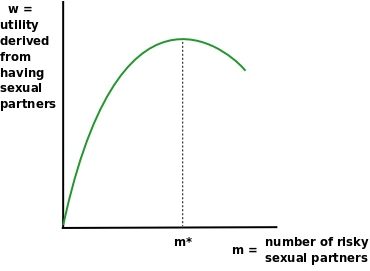
\includegraphics[scale=0.5]{sexutil.png}\end{center}
    \end{columns}
}

\subsection{HIV Transmission}
\frame
{
  \ft{HIV Transmission}
  \bi
  \item Probability of contracting HIV in period $t$, die before $t+1$: $\pi(m_t) = 1 - (1-ht)^{m_t}$
    \bi
    \item $h \in (0,1)$ be the HIV prevalence among potential partners.
    \item $t \in (0,1)$ be the female-to-male transmission rate (per partnership).
    \item For a given partner, probability of not contracting HIV: $(1-ht)$.
    \item For $m_t$ partners: $(1-ht)^{m_t}$.
    \ei
  \item What this means?  Probability of contracting HIV increases as...
    \bi
    \item HIV prevalence among partners increases.
    \item Transmission rate increases.
    \item Number of sexual partners increases.
    \ei
  \ei
}

\subsection{Optimization Problem}
\frame
{
  \ft{Expected Life-Cycle Utility}
  Expected utility over three periods:
  \bdm \begin{array}{l} \ds U = u(c_1, f_1, m_1) + \beta (1-\delta)\left[1-\pi(m_1)\right] u(c_2, f_2, m_2) \\\\ 
  \ds + \beta \left\{1 - (1-\delta)\left[1-\pi(m_1)\right] \right\} u(0,f_2,0) \\ \\
  \ds + \beta^2 (1-\delta)^2 \left[1-\pi(m_1)\right]\left[1-\pi(m_2)\right] u(c_3, f_3, 0) \\ \\
  \ds + \beta^2 \left\{1 - (1-\delta)^2 \left[1-\pi(m_1)\right]\left[1-\pi(m_2)\right]\right\} u(0, f_3, 0) \end{array} \edm


}

\frame
{
  \ft{Expected Life-Cycle Budget Constraint}
  Expected budget constraint over three periods:
\bdm \begin{array}{l} \ds p_1(c_1 + f_1) + (1-\delta) \left[1-\pi(m_1)\right] \frac{p_2 c_2}{1+r} + \frac{p_2 f_2}{1+r} \\ \\
\ds + (1-\delta)^2 \left[1-\pi(m_1)\right] \left[1-\pi(m_2)\right] \frac{p_3 c_3}{\left(1+r\right)^2}+ \frac{p_3 f_3}{\left(1+r\right)^2} \\ \\
\ds = w_1 + (1-\delta) \left[1-\pi(m_1)\right] \frac{w_2}{1+r}+ \delta \left[1-\pi(m_1)\right] \frac{b_2}{1+r} \\ \\
\ds + \delta (1-\delta) \left[1-\pi(m_1)\right] \left[1-\pi(m_2)\right] \frac{b_3}{(1+r)^2} \end{array} \edm

  \bi
  \item $w_1$, $w_2$ are incomes earned during periods 1 and 2.
  \item $b_2$, $b_3$ are possible life insurance payouts.
  \ei
}

\section{Results}
\subsection{Parameters}
\frame
{
  \ft{Solving the Model}
  \bi
  \item The model has no closed form solution.
  \item For a given set of parameters, can use numerical methods and computing power.
  \item Simulate the model for a large range of parameters for...
    \bi
    \item life expectancy (determines $\delta$, the probability of dying from something other than AIDS),
    \item income (assume $w_1=w_2$),
    \item size of life insurance benefit (assume $b_1=b_2$),
    \item elasticity of substitution for personal / family consumption, $\nu$.
    \item preference for personal over family consumption, $\alpha$.
    \ei
  \ei
}

\frame
{
  \ft{Baseline Parameters}
  \bi
  \item Data is not available for Sub-Saharran countries to estimate this model. 
  \item Some parameters are set to match situation in Zambia:
    \bi
    \item Overall HIV Prevalence among women (potential partners): $h = 0.161$.
    \item Income over 15 years for a family of 4: $w_1=w_2=$ \$22,440 (US dollars, constant 2000 prices).
    \item Exogenous probability of dying: $\delta = 0.508$\\(Non-AIDS life expectancy for men 51 years).
    \ei
  \item Other parameters we have good guesses for:
    \bi
    \item Transmission rate: $t=0.15$.
    \item Interest rate / Discount rate (15 year period):\\$r=0.82$, $\beta=0.547$.
    \ei
  \ei
}

\frame
{
  \ft{Baseline Preference Parameters}
  \bi
  \item Some utility function parameters we just completely make up:
    \bi
    \item Personal consumption preference parameter: $\alpha=0.5$.
    \item Elasticity of substitution personal/family consumption: $\nu=1.0$.
    \item Satiation point: $m^* = 50$.
    \ei
  \item Set the utility function sexual partners to match HIV prevalence rates among men in Zambia:
    \bi
    \item $\gamma_1 = 1.360$, leads to HIV prevalence among men ages 25-39, $\pi(m_1)=0.170$.
    \item $\gamma_2 = 0.501$, leads to HIV prevalence among men ages 40-54, $\pi(m_2)=0.142$.
    \ei
  \ei
}

\subsection{Dynamics of Risky Behavior}
\frame
{
  \ft{HIV Prevalence: Life Expectancy}
  \begin{center}
  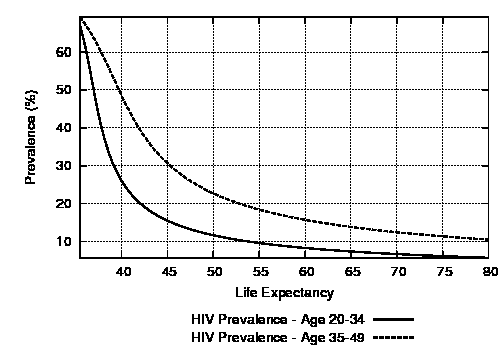
\includegraphics[scale=0.32]{images/hivlife.png} 
  \end{center}
  \vspace*{-0.2in}
  \bi
  \item HIV prevalence among adult men can decrease from 17\% (young) and 14\% (middle-age) to about 7\%.
  \item Shortening life expectancy can result in big increases in HIV prevalence.
  \item Likely \textit{under-estimates} true effect, since $h$ remains constant ($h=0.161$).
  \ei
}

\frame
{
  \ft{HIV Prevalence: Income}
  \begin{center}
  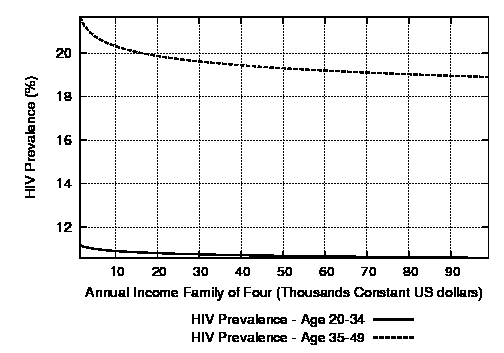
\includegraphics[scale=0.32]{images/hivgdp.png} 
  \end{center}
  \vspace*{-0.2in}
  \bi
  \item Smaller responses to increases in income.
  \item For Age 25-39, possible decrease in prevalence from 17\% to about 15.7\% (7.6\% reduction in men with HIV).
  \item For Age 40-54, possible decrease in prevalence from 14.2\% to about 12.3\% (13.4\% reduction in men with HIV).
  \ei
}

\frame
{
  \ft{HIV Prevalence: Income}
  \bi
  \item Deterrence effect of higher income is not as great as deterrence effect of longer non-AIDS life expectancy.
  \item Two effects of an increase in income
  \item Substitution effect: causes a decrease in risky behavior (greater opportunity cost to risky behavior).
  \item Income effect: causes an increase in risky behavior (greater ability to pay for all goods).
  \item Substitution effect is small when life expectancy is short, this is why effect on income is so small.
  \ei
}

\frame
{
  \ft{HIV Prevalence: Life Expectancy and Income}
  \vspace*{-0.35in}
  \begin{center}
    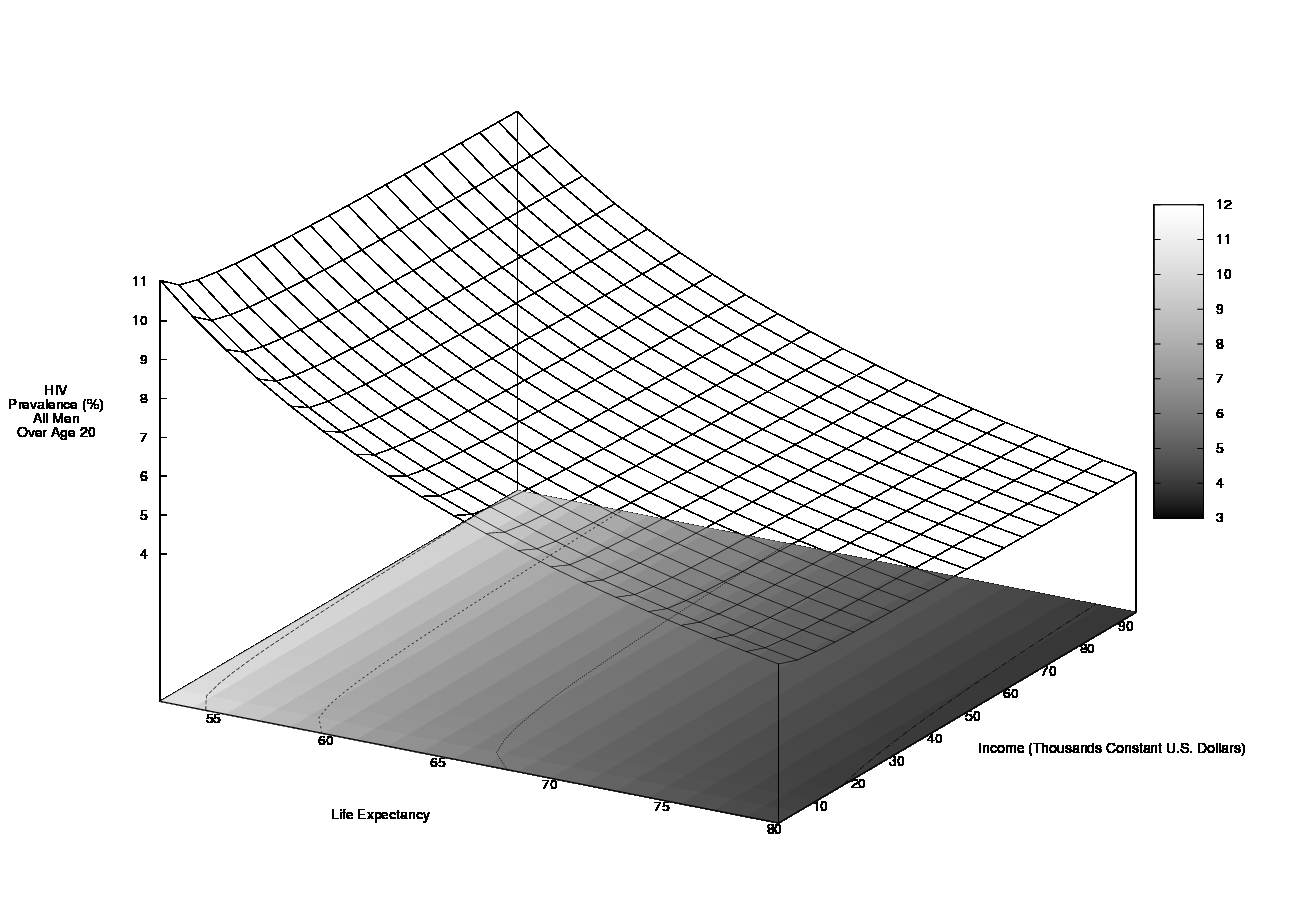
\includegraphics[scale=0.3]{images/hiv_gdplife.png}
  \end{center}
}

\frame
{
  \ft{HIV Prevalence: Life Expectancy and Income}
  \bi
  \item Increased life expectancy can be a large deterrent to risky behavior.
  \item Increased income is a relatively smaller deterrent.
  \item Deterrence effects of life expectancy and income complement each other.
  \item Can life insurance payouts replicate these effects?
    \bi
    \item Notice: utility functions value family consumption even after a possible death.
    \ei
  \ei
}

\frame
{
  \ft{HIV Prevalence: Life Insurance Benefit}
  \begin{center}
  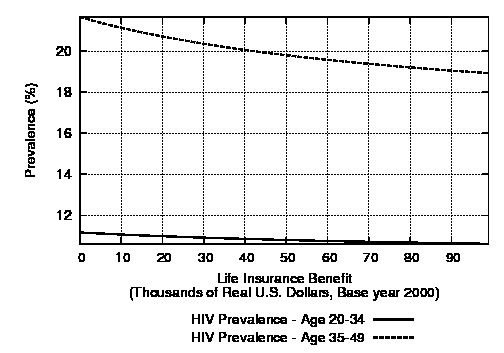
\includegraphics[scale=0.32]{images/hivB.png} 
  \end{center}
  \bi
  \item Life insurance benefit mirrors effect of income, not so much life expectancy.
  \ei
}

\subsection{Life Insurance and Preference Parameters}
\frame
{
  \ft{Determinants of Life Insurance Effectiveness}
  \bi
  \item Uncertain calibrations for: 
    \bi
    \item Preference for personal over family consumption, $\alpha$.
    \item Substitutability of personal and family consumption, $\nu$.
    \ei
  \item Life insurance should be more effective if...
    \bi
    \item individuals care more about family consumption (lower $\alpha$).
    \item family and personal consumption are more highly substitutable (higher $\nu$).
    \ei
  \ei
}

\frame
{
  \ft{Life Insurance: Value for Personal Consumption}
  \vspace*{-0.35in}
  \begin{center}
    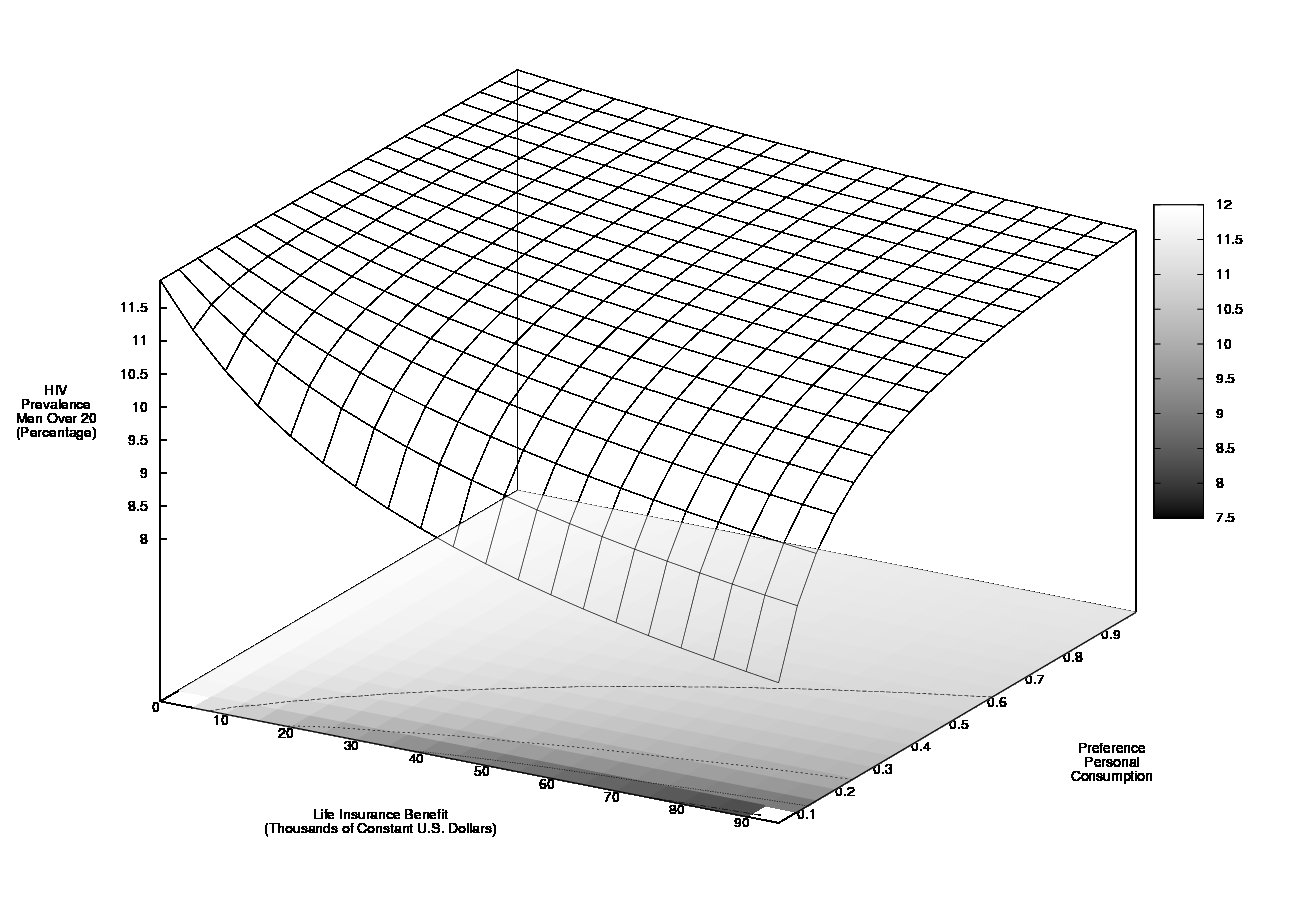
\includegraphics[scale=0.3]{images/hivBalpha.png}
  \end{center}
}

\frame
{
  \ft{Life Insurance: Value for Personal Consumption}
  \bi
  \item As $\alpha$ gets larger, the \textit{greater} is deterrence effect of an \textit{increase in income} (not shown).
    \bi
    \item Increases substitution effect: greater selfishness increases the opportunity cost of risky behavior.
    \ei
  \item However, as $\alpha$ gets larger, the \textit{smaller} is going to be the effectiveness of life insurance benefits.
    \bi
    \item Life insurance is paid out only if dead and can only finance family consumption.
    \ei
  \ei
}

\frame
{
  \ft{Life Insurance: Elasticity of Substitution}
  \vspace*{-0.35in}
  \begin{center}
    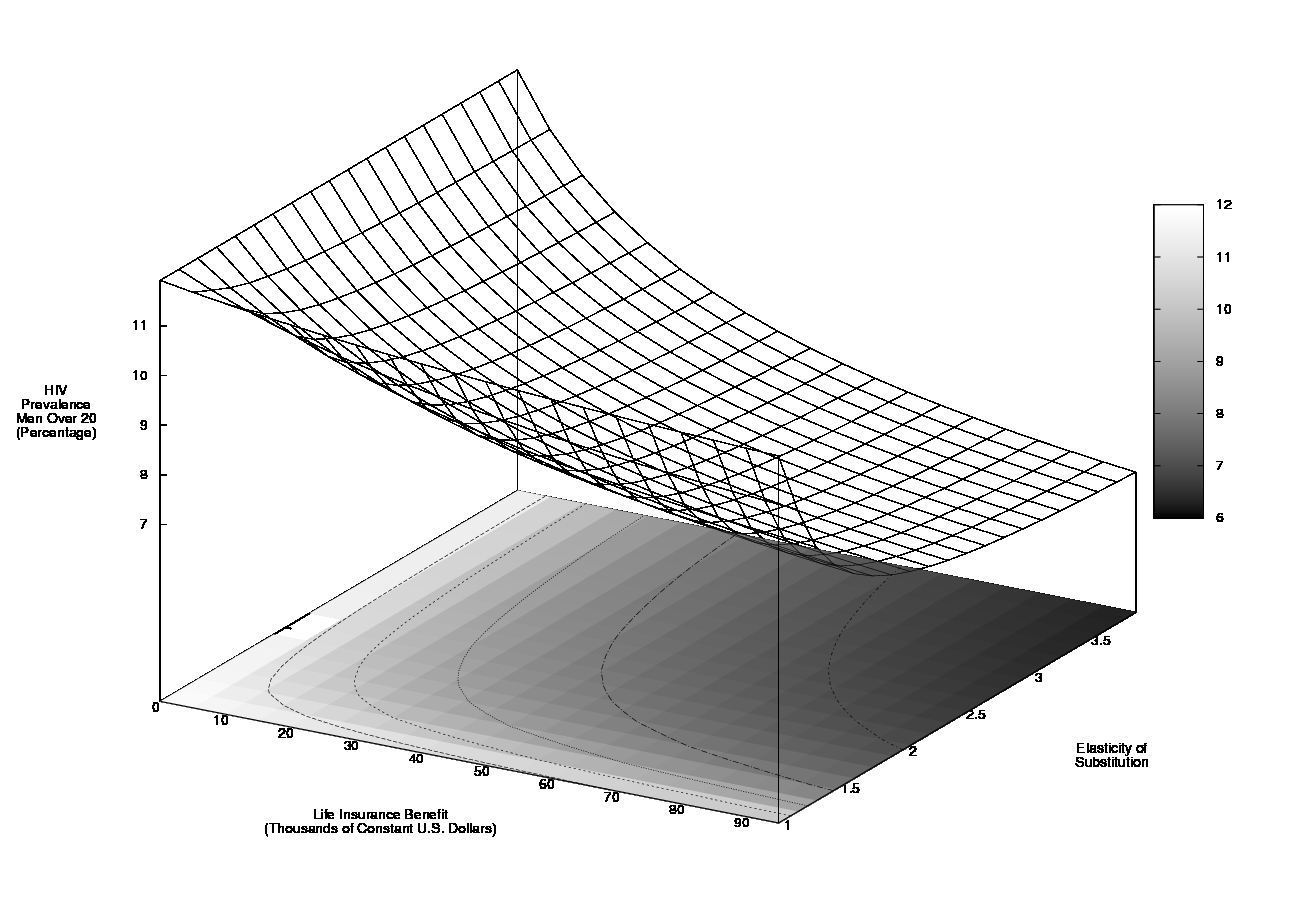
\includegraphics[scale=0.3]{images/hivBsub.png}
  \end{center}
}

\frame
{
  \ft{Life Insurance: Elasticity of Substitution}
  \bi
  \item As $\nu$ gets larger, the \textit{smaller} is deterrence effect of an \textit{increase in income} (not shown).
    \bi
    \item Decreases the substitution effect: family consumption (which can be enjoyed when dead) makes a suitable substitute for personal consumption.
    \ei
  \item However, as $\nu$ gets larger, the \textit{greater} is going to be the decrease in risky sexual activity and HIV prevalence in response to an \textit{increase in income}.
    \bi
    \item If family consumption (can be enjoyed if dead) and personal consumption (only if alive) are highly substitutable, life insurance can have a similar effect of increasing life expectancy.
    \ei
  \ei
}

\frame
{
  \ft{Discovering Preference Parameters}
  \bi
  \item Finding evidence or computing estimates for preference parameters is left for future research.
  \item Interview evidence may shed light on $\alpha$ (value of personal vs family consumption).
  \item If people in countries with higher incomes but low life expectancies have little differences in risky sexual behavior:
    \bi
    \item $\alpha$ is likely small (greater value for family consumption).
    \item $\nu$ is likely large (family and personal consumption are highly substitutable).
    \item Perhaps counter-intuitively, the \textit{more} effective will be a government provided life-insurance policy.
    \ei
  \ei
}

\section{}
\subsection{Conclusion}
\frame
{
  \ft{Conclusion}
  \bi
  \item Life-cycle model
    \bi
    \item Low life expectancy and low income leads to highly risky behavior.
    \item High life expectancy and high income leads to much safer behavior.
    \ei
  \item Life insurance can replicate small effects of a high income.
  \item Life insurance can replicate large effects of \textit{both} a high income and high life expectancy,
    \bi
    \item if value for personal consumption versus family consumption is low and/or
    \item if elasticity of substitution between personal and family consumption is high.
    \ei
  \item Easy for life insurance deterrent to have large coverage.
  \item Should encourage HIV testing, complement existing prevention measures.
  \ei
}

\end{document}

